  \subsection{View a live run}
A User can view a run live through his/her device, visualizing the map in which the run is being performed and the relative locations of each partecipant.

\begin{table}[H]
	\centering
    
    \begin{tabular}{|p{3.5cm}|p{10.3cm}|}
    
    \hline
    \textbf{\large{Actors}}  			& \tabitem User 	\\
    				 					
    \hline
    \textbf{\large{Goals}} 				& \ref{goal:run4};\\
    
    \hline
    \textbf{\large{Enter Condition}}	& The \emph{User} has already visualize the list of live runs.		\\
    
    \hline
    \textbf{\large{Events Flow}}		& \begin{enumerate}[leftmargin=0.5cm]
                                          	\item The \emph{User}  selects the run that wants to view
                                            \item The System shows the details about the run (location, date, time, number of partecipants, online spectators)
                                             \item The \emph{User} can select the 'View Live' button to visualize the map of the run and the live location of each partecipant
                                            \item The System shows the map with the partecipants locations and increments the number of online spectators
                                           
                                          \end{enumerate}
    										\\
    \hline
    \textbf{\large{Exit Conditions}}    & The User visualizes the run and the number of online spectators in incremented.  \\
    
    \hline
    \textbf{\large{Exceptions}} 		& \\
    
    \hline
    
    
    \end{tabular}
	
\end{table}

\begin{figure}[H]
    \centering
    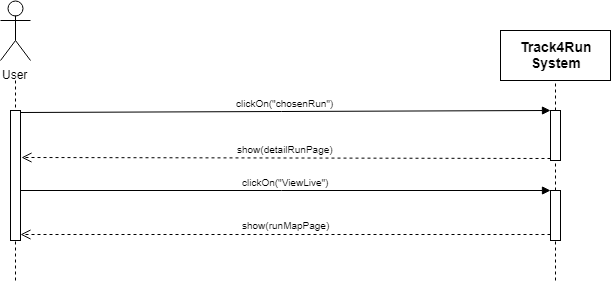
\includegraphics[scale=0.4]{Pictures/viewLiveRun.png}
    \caption{State chart  \emph{Data4Help} System}
\end{figure}
